
% Morten -- jeg skriver bare en veldig plain tex-fil her, så kan du gjøre det du vil med innholdet etterpå.


\documentclass{article}
\usepackage[utf8]{inputenc}
\usepackage[a4paper]{geometry}
\usepackage[norsk]{babel}
\usepackage{amssymb}
\usepackage{amsmath}
\usepackage{amsthm}
\usepackage{multicol}
\usepackage{scrextend}
\usepackage{mdframed}
\usepackage{hyperref}
\usepackage{listings}
\usepackage{tikz}
\usetikzlibrary{patterns,decorations.pathmorphing}
\usetikzlibrary{arrows.meta}
\usepackage{pgfplots}
\usepackage{array}
\usepackage{mdframed}
\usepackage[american]{circuitikz}
\usepackage[small]{titlesec}

\hypersetup{colorlinks=true, 
    linkcolor=blue, 
    filecolor=magneta,
    urlcolor=cyan,
    citecolor=black,
}

\theoremstyle{plain}
\newtheorem{teorem}{Teorem}\surroundwithmdframed{teorem}

\theoremstyle{definition}
\newtheorem{definisjon}[teorem]{Definisjon}
\newtheorem{eksempel}[teorem]{Eksempel}
\newtheorem{funfact}[teorem]{Funfact}

\theoremstyle{remark}
\newtheorem{merknad}[teorem]{Merknad}
\newtheorem*{bevis}{Bevis}

\newtheorem{oppg}{}
\newtheorem{innercustomoppg}{}
\newenvironment{customoppg}[1]
{\renewcommand\theinnercustomoppg{#1}\innercustomoppg}
{\endinnercustomoppg}

% Endre på disse etter hvilken notasjon du vil ha.
\newcommand{\diff}[1]{\mathop{d#1}} 
\newcommand{\fcn}{x}
\newcommand{\boldvec}[1]{\boldsymbol{\mathrm{#1}}}
\newcommand{\expfcn}[1]{e^{#1}}
\newcommand{\bigabs}[1]{\big|#1\big|}
\newcommand{\biggabs}[1]{\bigg|#1\bigg|}
\newcommand{\bigparanth}[1]{\big(#1\big)}
\newcommand{\biggparanth}[1]{\bigg(#1\bigg)}
\newcommand{\bigbrac}[1]{\big[#1\big]}
\newcommand{\biggbrac}[1]{\bigg[#1\bigg]}
\newcommand{\imagunit}{\mathrm{j}}

\DeclareMathOperator{\imaginary}{Im}
\DeclareMathOperator{\real}{Re}


\title{Ikkelineære systemer}
\author{}
\date{}

\begin{document}
\maketitle

Dette kapitlet gir en introduksjon til dynamiske systemer. Mens vi tidligere har sett at det finnes god teori og fine formler for lineære systemer gjelder ikke dette for ikkelineære systemer. For ikkelineære systemer kan man som regel ikke finne analystiske løsninger, og vi må bruke andre metoder. Disse inkluderer hovedsaklig kvalitative argumenter i fasediagrammet og numerisk analyse.

\begin{eksempel}
    Som et eksempel på at forståelse noen ganger kan være mer nyttig enn eksakte formler begynner vi med å betrakte ligningen
    \begin{equation} \label{eks:motiverende_eksempel}
        \dot{\fcn}(t) = \sin(\fcn(t)).
    \end{equation}
    Her er $x(t)$ en funksjon av variabelen $t$, og $\dot{x}$ er den deriverte av funksjonen. Dette er en ikkelineær førsteordens differensialligning. Løsningen kan vi finne ved separasjon. Først skriver vi ligningen på formen
    \begin{equation*}
        \frac{1}{\sin(\fcn(t))} \frac{\diff{\fcn(t)}}{\diff{t}} = 1.
    \end{equation*}
    Nå kan vi bruke formelen
    \begin{equation*}
        \int \frac{1}{\sin(\fcn)} \diff{\fcn} = -\ln(\csc(\fcn) + \cot(\fcn))
    \end{equation*}
    for den antideriverte av $1/\sin(\fcn)$ (du trenger ikke å regne ut dette) og kjerneregelen til å skrive ligningen som
    \begin{equation*}
        \frac{\diff{}}{\diff{t}} \bigparanth{-\ln(\csc(\fcn) + \cot(\fcn))} = 1.
    \end{equation*}
    Integrasjon med initialbetingelse $\fcn = \fcn_0$ i $t = 0$ gir da den implisitte løsningen
    \begin{equation} \label{eq:motiverende_eksempel_losn}
        t = \ln \biggabs{ \frac{\csc(\fcn_0) + \cot(\fcn_0)}{\csc(\fcn) + \cot(\fcn)}}.
    \end{equation}
    Selv om dette er en av få ikkelineære differensialligningen man kan finne analytisk løsning til var denne utregningen vanskelig, og enda vanskeligere er det å tolke løsningen \eqref{eq:motiverende_eksempel_losn}. Kan vi forstå ligningen på andre måter?
    
    Vi kan tenke oss at $\fcn(t)$ beskriver posisjonen til en partikkel som beveger seg langs den reelle tallinjen. Ligning \eqref{eks:motiverende_eksempel} gir da at hastigheten til partikkelen er avhengig av en sinusfunksjon med partikkelens posisjon som argument. Under er en skissere av det endimensjonale fasediagrammet til ligningen.
    \begin{center}
        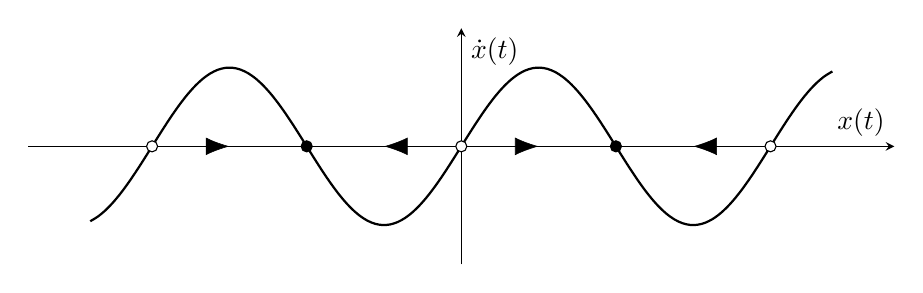
\begin{tikzpicture}
            \pgfplotsset{ticks=none},
            \begin{axis} [
                ymax=1.5,
                ymin=-1.5,
                xmax=11,
                xmin=-11,
                x=0.5cm,
                y=1cm,
                axis lines=center,
                trig format plots=rad,
                ylabel={$\dot{\fcn}(t)$},
                xlabel={$\fcn(t)$}
                ]
                \addplot [domain=-3*pi:3*pi, samples=100, smooth, thick] { sin(0.8*x) };

                \draw[-{Latex[length=3mm]}, very thin] (axis cs:-2*pi/0.8,0) -- (axis cs:-3*pi/1.6,0);
                \draw[-{Latex[length=3mm]}, very thin] (axis cs:0,0) -- (axis cs:-pi/1.6,0);
                \draw[-{Latex[length=3mm]}, very thin] (axis cs:2*pi/0.8,0) -- (axis cs:3*pi/1.6,0);
                \draw[-{Latex[length=3mm]}, very thin] (axis cs:0,0) -- (axis cs:pi/1.6,0);
                
                \node[circle, draw=black, fill=white, inner sep=0pt, minimum size=4pt] at (axis cs:-2*pi/0.8,0) {};
                \node[circle, draw=black, fill=black, inner sep=0pt, minimum size=4pt] at (axis cs:-pi/0.8,0) {};
                \node[circle, draw=black, fill=white, inner sep=0pt, minimum size=4pt] at (axis cs:0,0) {};
                \node[circle, draw=black, fill=black, inner sep=0pt, minimum size=4pt] at (axis cs:pi/0.8,0) {};
                \node[circle, draw=black, fill=white, inner sep=0pt, minimum size=4pt] at (axis cs:2*pi/0.8,0) {};
                
            \end{axis}
          \end{tikzpicture}
    \end{center}
    I punktene der sinusfunksjonen er positiv er hastigheten til partikkelen positiv, der den er negativ er hastigheten negativ, og der funksjonen krysser null er også hastigheten til partikkelen null. Punktene hvor hastigheten er null, og dermed partikkelen er i ro, kalles likevektspunkter. Vi klassifiserer gjerne likevektspunktene som enten stabile eller ustabile, avhengig av hva som skjer dersom en partikkel i et likevektspunkt får et lite dytt på seg. De ustabile likevektspunktene er tegnet inn som hvite punkter mens de stabile er svarte.
    
    Ut fra diagrammet kan vi se hvordan partikkelen vil bevege seg. Dersom den begynner i posisjon $x_0$ beveger den seg til et likevektspunkt til høyre eller til venstre, avhengig at om hastigheten er positiv eller negativ.
\end{eksempel}

Eksempel \ref{eks:motiverende_eksempel} viser hvordan det ofte kan være nyttig å skissere faseplanet til en ligning i stedet for å lete etter eksakte løsninger. På denne måten kan vi få mer informasjon ut av systemet for mindre arbeid.


\section*{Todimensjonale fasediagram}
Vi skal nå se litt på todimensjonale fasediagram. For lineære systemer på formen
\begin{equation*}
    \boldvec{\dot{x}}(t) = A \boldvec{x}(t)
\end{equation*}
kan man, med litt erfaring, skissere fasediagrammet bare ved å se på egenskapene til matrisen $A$ i systemet. Vi ser nå på noen eksempler på dette.

\begin{eksempel}
    Betrakt systemet
    \begin{equation*}
        \dot{x} = x - 5 y, \qquad \dot{y} = x - y.
    \end{equation*}
    Matrisen
    \begin{equation*}
        \begin{pmatrix}
            1 & -5 \\
            1 & -1
        \end{pmatrix}
    \end{equation*}
    har komplekse egenverdier $\lambda_1 = 2 \imagunit$ og $\lambda_2 = -2 \imagunit$. Vi får derfor sirkelbaner i faseplanet, som vist under.
    \begin{center}
        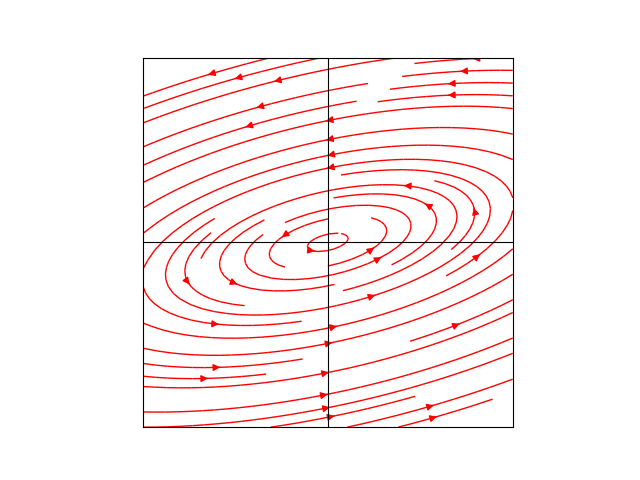
\includegraphics[scale=0.5]{phase_plane_2.png}
    \end{center}
\end{eksempel}

\begin{eksempel}
    Se nå på systemet
    \begin{equation*}
        \dot{x} = x + y, \qquad \dot{y} = x - 2y.
    \end{equation*}
    Matrisen
    \begin{equation*}
        \begin{pmatrix}
            1 & 1 \\
            1 & -2
        \end{pmatrix}
    \end{equation*}
    har reelle egenverdier $\lambda_1 = \frac{1}{2} (-1 - \sqrt{13})$ og $\lambda_2 = \frac{1}{2} (-1 + \sqrt{13})$ med tilhørende reelle egenvektorer. Vi får da en sadel i faseplanet, bestemt av linjene til egenverdiene for systemt.
    \begin{center}
        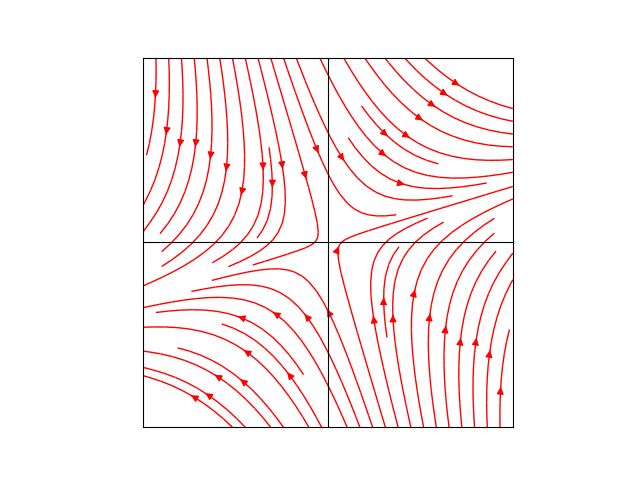
\includegraphics[scale=0.5]{phase_plane_3.png}
    \end{center}
\end{eksempel}

\begin{eksempel} \label{eks:lodd_svingning}
    Vi har tidligere sett at dersom et lodd henger i en fjær som vist under kan svingningen til loddet beskrives av
    \begin{equation*}
        m \ddot{x} + \gamma \dot{x} + k x = 0,
    \end{equation*}
    der $m$ er massen til loddet, $\gamma$ er en friksjonskoeffisient, og $k$ er fjærstivheten.
    \begin{center}
        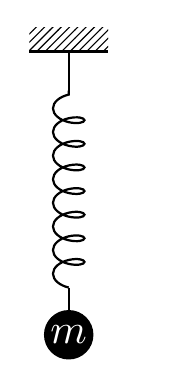
\begin{tikzpicture}[thick,
            every node/.style = {draw      = none,
                                inner sep = 0pt,
                                outer sep = 0pt},
            platform/.style   = {fill,
                                pattern = north east lines,
                                minimum width  = 1cm,
                                minimum height  =0.3cm}
            ]
            \newcommand{\springfig}[6]{%
            \begin{scope}[xshift=#6,
                        spring/.style = {decorate,
                                        decoration = {aspect         = 0.5, 
                                                        segment length = #1,
                                                        amplitude      = 2mm,
                                                        coil}}]
            
            \path (0,0)                            coordinate (g) 
                (0,-0.5cm)                       coordinate (topspring) 
                (0, #2)                          coordinate (bottomspring) 
                (bottomspring) ++(0,-.3cm)       coordinate (pt2)
                                +(0cm,-#3)       coordinate (pt3)
                                +(1.25cm,-#3)    coordinate (#5 pt3);
            
                \node [platform,
                    anchor = south] at (g)  {};
                \draw [very thick]    (-0.5,0)         -- (0.5,0);
                \draw                (topspring)     -- (g)
                                    (bottomspring)  -- (pt2.north);
                \draw [spring]       (bottomspring)  -- (topspring);
                \draw [fill=black] (pt3) circle (#3) 
                                        node[inner sep = 0,
                                                scale     = #4,
                                                text      = white]{$m$};
                \end{scope}
            }
            \springfig{3mm}{-3cm}{0.3cm}{1.5}{A}{0cm}
            \end{tikzpicture}  
        \end{center}
    Desom vi innfører den nye funksjonen $y(t) = \dot{x}(t)$ for hastigheten til loddet kan ligningen skrives om til systemet
    \begin{equation*}
        \begin{pmatrix}
            \dot{x} \\
            \dot{y}
        \end{pmatrix}
        =
        \begin{pmatrix}
            0 & 1 \\
            -\frac{k}{m} & -\frac{\gamma}{m}
        \end{pmatrix}
        \begin{pmatrix}
            x \\
            y
        \end{pmatrix}
    \end{equation*}
    For enkelhets skyld velger vi verdier $m = 1$, $\gamma = 2$ og $k = 5$. Matrisen
    \begin{equation*}
        \begin{pmatrix}
            0 & 1 \\
            -5 & -2
        \end{pmatrix}
    \end{equation*}
    har egenverdier $\lambda_1 = -1+2 \imagunit$ og $\lambda_2 = -1-2 \imagunit$, med tilhørende egenvektorer
    \begin{equation*}
        v_1 =
        \begin{pmatrix}
            -1 - 2 \imagunit \\
            5
        \end{pmatrix},
        \qquad v_2 =
        \begin{pmatrix}
            -1 + 2 \imagunit \\
            5
        \end{pmatrix},
    \end{equation*}
    Tidligere har vi sett at systemet da har to lineært uavhengige løsninger på formen $v_1 \expfcn{\lambda_1 t}$ og $v_2 \expfcn{\lambda_2 t}$. Dette gir løsningene
    \begin{equation*}
        \begin{pmatrix}
            -1 - 2 \imagunit \\
            5
        \end{pmatrix}
        \expfcn{(-1 + 2 \imagunit) t} \qquad \textnormal{og} \qquad
        \begin{pmatrix}
            -1 + 2 \imagunit \\
            5
        \end{pmatrix}
        \expfcn{(-1 - 2 \imagunit) t}.
    \end{equation*}
    Videre kan vi bruke superposisjonsprinsippet til å skrive den generelle løsningen til systemet på formen
    \begin{equation*}
        \begin{pmatrix}
            x(t) \\
            y(t)
        \end{pmatrix}
        = c_1 \biggbrac{
            \begin{pmatrix}
                -1 \\
                5
            \end{pmatrix}
            \cos(2t) +
            \begin{pmatrix}
                -2 \\
                0
            \end{pmatrix}
            \sin(2t)
        } \expfcn{-t} + c_2 \biggbrac{
            \begin{pmatrix}
                -1 \\
                5
            \end{pmatrix}
            \sin(2t) +
            \begin{pmatrix}
                -2 \\
                0
            \end{pmatrix}
            \cos(2t)
        } \expfcn{-t},
    \end{equation*}
    der $c_1$ og $c_2$ er to konstanter som kan bestemmes av eventuelle initialbetingelser. Ut fra dette kan vi lese at systemet inneholder periodiske svingninger, men at disse dempes av $\expfcn{-t}$-funksjonen i løsningen.
    
    Følgende viser fasediagrammet for systemet, med $x(t)$ på den horisontale aksen og $y(t)$ på den vertikale aksen.
    \begin{center}
        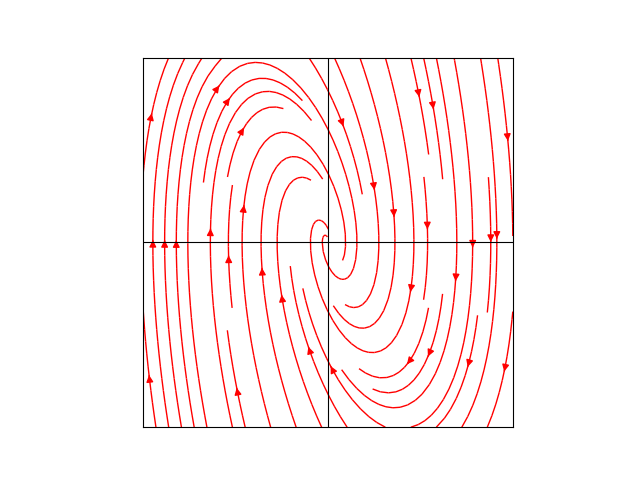
\includegraphics[scale=0.5]{phase_plane_1.png}
    \end{center}
    Her finner vi det vi forventet; posisjonen til loddet $x(t)$ og hastigheten til loddet $y(t)$ beveger seg periodisk i forhold til hverandre samtidig som begge dempes inn mot null av friksjon. Ingen energi blir tilført systemet, som derfor til slutt vil komme til stillstand.
\end{eksempel}

I fasediagrammet plotter vi løsningene mot hverandre, i motsetning til å plotte dem hver for seg som funksjoner av tid. Tiden $t$ er dermed implisitt i diagrammet. Hvert punkt i planet tilsvarer én tilstand systemet kan befinne seg i, hvor både posisjon og hastighet er bestemt. Kurver i fasediagrammet er spesielle løsninger til systemet, hvor konstantene i den generelle løsningen er bestemt av initialbetingelser.

\section*{Grensesykler}

Vi går nå over til å studere systemer som ikke er lineære. I disse kan man få helt andre fenomener enn de vi tidligere har sett i lineære systemer. Her kommer også analyse av faseplan til sin rett, i og med at vi som regel ikke kan løse slike systemer analytisk. La oss først se på to situasjoner hvor ikkelineære ligninger oppstår.

\begin{eksempel}    
    I Eksempel \ref{eks:lodd_svingning} så vi på fasediagrammet til ligningen
    \begin{equation*}
        m \ddot{x} + \gamma \dot{x} + k x = 0.
    \end{equation*}
    Siden det er friksjon i systemet dør svingningen ut til slutt. La oss nå tenke oss at vi begynner å gi loddet litt fart i hver svingning. Det at vi dytter på loddet kan vi modellere med negativ friksjon; vi tilfører systemet energi. Nå kan svingningen holdes i gang så lenge vi orker å dytte på loddet. Men systemet er ikke lenger lineært, siden friksjonen ikke er proporsjonal med hastigheten. Vi kan sette opp ligningen
    \begin{equation} \label{eq:ikkelin_fjær}
        m \ddot{x} + \gamma(x) \dot{x} + k x = 0,
    \end{equation}
    der $\gamma(x)$ gir friksjon som funksjon av posisjonen til partikkelen.
\end{eksempel}


\begin{eksempel}
    Betrakt følgende krets.
    \begin{center}
        \begin{circuitikz}
          \draw
          (0,0)
          to[american voltage source, voltage dir=old, l={$V_s$}, i^={$I(t)$}] (0,3)
          to[european resistor, l_ = ${V=f(I)}$] (3,3)
          to (3,0)
          to[cute inductor, l_ = $L$] (0, 0);
        \end{circuitikz}
      \end{center}



\end{eksempel}


Vi skal se på ett av disse her, nemlig grensesykler. En grensesyklus er en lukket og isolert bane i et fasediagram. Systemer som inneholder grensesykler finner vi overalt rundt oss. Noen eksempler er kretsen i en digital klokke, et hjerte som slår, eller balansen mellom rovdyr og byttedyr.

\begin{eksempel}
    Dersom vi bruker polarkoordinater er det ikke vanskelig å konstruere systemer som har grensesykler. Gitt ved
    \begin{equation*}
        x = r \cos(\theta), \qquad y = r \sin(\theta).
    \end{equation*}
    Deriverer vi får man
    \begin{equation*}
        \dot{r} = \frac{x\dot{x} + y \dot{y}}{r}, \qquad \dot{\theta} = \frac{x\dot{y} - \dot{x}y}{r^2}.
    \end{equation*}
    Ta for eksempel
    \begin{equation*}
        \begin{pmatrix}
            \dot{r} \\
            \dot{\theta}
        \end{pmatrix}
        =
        \begin{pmatrix}
            r(1-r^2) \\
            1
        \end{pmatrix}
    \end{equation*}
    hvor $r$ er radiusen fra origo i planet og $\theta$ beskriver vinkelen fra den horisontale aksen. Siden $r(1-r^2)$ har nullpunkt i $r = 1$ har vi en grensesyklus i $r = 1$.
    \begin{center}
        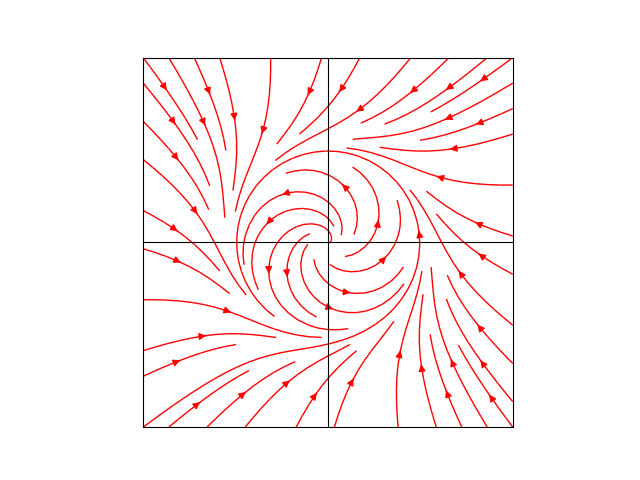
\includegraphics[scale=0.5]{phase_plane_radial.png}
    \end{center}
\end{eksempel}

\begin{eksempel}
    Krets for Van der Pol.
    \begin{center}
        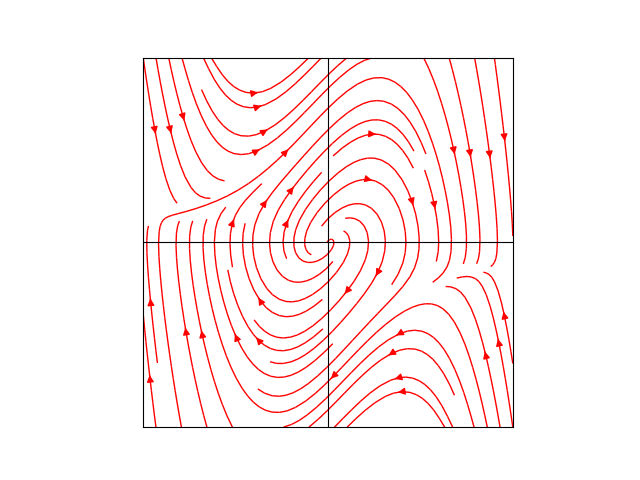
\includegraphics[scale=0.5]{van_der_pol.png}
    \end{center}
\end{eksempel}

Vi trenger likevel ikke å bruke polarkoordinater for å forstå hvordan grensesykler kan oppstå. Tenk nå på eksempel \ref{eks:lodd_svingning}, hvor vi hadde et lodd som svinget opp og ned i en fjær. Siden det er friksjon i systemet vil loddet til slutt stoppe av seg selv. Men hva vis vi begynner å dytte loddet litt oppover i hver svingning? Da vil vi ha tilført kraft i systemet, og vi kan se for oss at svingningen vil kunne fortsette så lenge vi har lyst til å sitte å dytte på loddet.


\begin{equation} \label{eq_lienard}
    \ddot{x} + f(x) \dot{x} + g(x) = 0.
\end{equation}

\begin{teorem}[Lienard's teorem]
    Dersom $f$ og $g$ tilfredsstiller følgende kriterier.
    \begin{enumerate}
        \item[(i)] $f$ og $g$ er kontinuerlig derivarbare.
        \item[(ii)] $g$ er en odde funksjon.
        \item[(iii)] $g(x) > 0$ for $x > 0$.
        \item[(iv)] $f$ er en jevn funksjon.
        \item[(v)] Funksjonen $F(x) = \int_0^x f(u) \diff{u}$ har nøyaktig ett nullpunkt $x = a$ for positive $x$. Videre er $F(x) < 0$ på $0 < x < a$ og $F(x) > 0$, $F'(x) \leq 0$ på $x > a$, med $F(x) \rightarrow \infty$ når $x \rightarrow \infty$.
    \end{enumerate}
    Da har Lienard-systemet en unik stabil grensesyklus rundt origo.
\end{teorem}

\begin{eksempel}
    Vi sjekker betingelsene for Van der Pol-ligningen
    \begin{equation*}
        \ddot{x} - \mu (1 - x^2) \dot{x} + x = 0.
    \end{equation*}
    Merk at denne er et spesialtilfelle av kretsen over.
\end{eksempel}

\section*{Numerisk analyse}

Vi skal ikke gå nøye gjennom teori her, men ta noen eksempler som viser at de samme metodene som vi har lært tidligere fungerer her også.

Ikkelineært eksempel. Van der Pol.


\section*{Oppgaver}

\begin{oppg}
    Skisser fasediagrammet til følgende lineære system.
    \begin{itemize}
        \item[(a)] $\dot{x} = x - 5y, \qquad \dot{y} = x - y$.
        \item[(b)] $\dot{x} = x + y, \qquad \dot{y} = x - 2y$.
        \item[(c)] $\dot{x} = 4x - 2y, \qquad \dot{y} = 3x - y$.
        \item[(d)] $\ddot{x} + 3\dot{x} + 2x = 0$.
        \item[(d)] $\ddot{x} - 4\dot{x} + 40x = 0$.
    \end{itemize}
    Hint: Se på egenverdiene og egenvektorene til matrisen som er assosiert med systemet. Dersom du er usikker kan fasediagrammet plottes ved hjelp av streamplot-funksjonen i python.
    \begin{lstlisting}
    % Lag et grid
    X, Y = np.meshgrid(
        np.linspace(-1.0, 1.0, 30), np.linspace(-1.0, 1.0, 30)
        )
    
    % Spesifiser hastighetene
    U = Y
    V = -5 * X - 2 * Y

    % Plot fasediagram
    plt.streamplot(
        X, Y, U, V, color="r", linewidth=1, density=1, minlength=0.25
        )
    
    % Valgfrie argumenter for et ryddig plot
    plt.axis("square")
    plt.xticks([], [])
    plt.yticks([], [])
    plt.axhline(color="black", lw=0.8)
    plt.axvline(color="black", lw=0.8)
    plt.show()

    \end{lstlisting}
\end{oppg}

\begin{oppg}
    Uttrykk systemet
    \begin{equation*}
        \left\{
            \begin{aligned}
                & \dot{x} = (x^2 + y^2 - 1)x + y, \\
                & \dot{y} = (x^2 + y^2 - 1)y - x,
            \end{aligned}    
        \right.
    \end{equation*}
    ved hjelp av polarkoordinater, og bruk dette til å argumentere for at systemet har en grensesyklus.
\end{oppg}

\begin{oppg}
    Se på ligningen
    \begin{equation*}
        \ddot{x} + (x^2 - 1) \dot{x} + \tanh(x) = 0
    \end{equation*}
    \begin{itemize}
        \item[(a)] Vis at den har en unik grensesykel.
        \item[(b)] Plot fasediagrammet til ligningen.
        \item[(c)] Finn numerisk løsning ved hjelp av symplektisk Euler.
    \end{itemize}
\end{oppg}

\begin{oppg}
    Se på ligningen
    \begin{equation*}
        \ddot{x} + \mu (x^4 - 1) \dot{x} + x = 0
    \end{equation*}
    \begin{itemize}
        \item[(a)] Vis at den har en unik grensesykel dersom $\mu > 0$.
        \item[(b)] Plot fasediagrammet til ligningen for $\mu = 1$.
        \item[(c)] Finn numerisk løsning ved hjelp av trapesmetoden.
    \end{itemize}
\end{oppg}


\end{document}